\chapter{Gradient Ascent}
\label{cha:gascent}

Beim Training von künstlichen neuronalen Netzwerken, wie etwa \ac{CNN}, werden die Gewichte $ w_{i} $ und der Schwellwerte (Bias) so lange verändert und im Modell des Netzwerks gespeichert, bis die Ausgabe aus dem Netzwerk die Eingabedaten (Trainingsbilder) annähern. 
Um zu quantifizieren, wie gut dieses Ziel erreicht wird, wird eine sogenannte Kostenfunktion (engl. cost function) definiert. 
Die Kostenfunktion geht also über jedes einzelne Bild aus dem Trainingsdatensatz und berechnet den Unterschied zwischen der gewünschten Ausgabe und dem Ausgabevektor $\vec{a}$ des Netzwerks.
Der Ausgabevektor $\vec{a}$ ist hierbei abhängig vom Eingabebild, dem Gewicht $w_{i}$ und dem Schwellwert.
Die Kostenfunktion hat den Wert 0 in etwa dann angenähert, wenn das Eingabebild annähernd dem Ausgabevektor $\vec{a}$ entspricht, was das Ziel des Trainings eines künstlichen neuronalen Netzwerks darstellt. Denn dann wurde das Eingabebild korrekt erkannt.
Im Rahmen des Trainings sollen also eine Reihe von Gewichten $w_{i}$ und Schwellwerten gefunden werden, welche zu einer minimalen Kostenfunktion führen. 
Dies wird erreicht mit dem Gradient Descent-Algorithmus\cite{zhou_understanding_2018}.
Dieser Algorithmus berechnet wiederholt den Gradienten und verbessert iterativ die Gewichte. 


Das \textit{Gradient Ascent}-Verfahren ist als Pendant zum Gradient Descent-Verfahren zu verstehen. Hier wird auf die berechneten Gradienten eines trainierten Convolutional Neural Networks zugegriffen und das Eingabebild so lange verändert, bis dies dem gewünschten Ergebnisbild entspricht.
\section{Konzept}
Um gegebene \ac{CNN} gezielt anzugreifen, das heißt Bilder zu erzeugen, die einer bestimmten Zielklasse entsprechen und gleichzeitig vom Menschen nicht als solche erkannt werden, eignet sich die Methode \textit{Targeted Backpropagation}, welche eine Variante des \textit{Gradient Ascent}-Verfahrens darstellt \cite{liu_delving_2016}.
Diese Methode setzt ein bereits trainiertes \ac{CNN} voraus, greift auf die Gradienten des Modells zu und verändert das Eingabebild – wie etwa ein zufallsgeneriertes Bild – so lange, bis es der gewünschten Zielklasse entspricht oder diese annähert. 
Bei diesem Verfahren kann man beobachten, dass relevante Pixel, welche die bedeutendsten Stellen im Bild repräsentieren, stärker mutiert werden als unwichtige Pixel, die weitgehend unverändert bleiben.
\section{Implementierung}

Zunächst wird als vorverarbeitender Schritt ein \ac{CNN} unter Verwendung der AlexNet Architektur in PyTorch trainiert. 
Die hierbei verwendete Architektur des AlexNet entstammt \cite{pytorch_datasets_2019} und wurde dahingehend modifiziert, dass das AlexNet zu Eingabebildern der Größe $64 \times 64$ Pixel, drei Farbkanälen (RGB) sowie zu den 43 Klassen aus dem \ac{GTSRB} Datensatz kompatibel ist. 
Die Bilder aus dem \ac{GTSRB} Trainingsdatensatz, welche unterschiedliche Bildgrößen aufweisen, wurden im Zuge des Trainings ebenfalls auf eine Bildgröße von 64 x 64 Pixel interpoliert. 
Das Training des AlexNet erfolgte 50 Epochen lang mit dem \ac{GTSRB} Trainingsdatensatz und erzielte mit dem \ac{SGD}-Optimierer eine Genauigkeit von annähernd 89\% (validiert mit dem \ac{GTSRB} Testdatensatz).
Die Implementierung des \textit{Gradient Ascent}-Verfahrens, unter Verwendung der \textit{Targeted Backpropagation}-Methode und dem trainierten AlexNet, erfolgte in einer modifizierten Variante zu \cite{ozbulak_pytorch_2019}. 

Unter Angabe der Zielklasse sowie der minimalen Zielkonfidenz erzeugt der Algorithmus zunächst ein Zufallsbild, welches als Eingabeparameter für das trainierte AlexNet verwendet wird. Unter Anwendung des SGD-Optimierers auf das Eingabebild werden die Gradienten entsprechend der spezifizierten Zielklasse berechnet. 

Diese Gradienten werden nicht verwendet, um die Parameter des AlexNet-Mo"-dells zu verändern, wie es beim Training der Fall war, sondern um das eingegebene Bild dahingehend zu modifizieren, dass es der gewünschten Zielklasse entspricht. 
Die entsprechenden Pixel der aktivierten Neuronen werden hierzu (je nach Aktivierungsstärke) mit den Bildpixelwerten addiert. 
Dieser Prozess wird so lange wiederholt, bis das veränderte Bild die gewünschte Konfidenz zu der angegebenen Zielklasse erreicht hat.

Der Algorithmus wurde für jede der 43 \ac{GTSRB}-Klassen so lange wiederholt, bis das veränderte Bild die gewünschte Mindest-Konfidenz von 100\% erreicht.
Zur abschließenden Evaluierung der erzeugten Bilder am \ac{NN} des \ac{GI}-Wettbewerbs, werden alle Bilder an das Webinterface des Wettbewerbs gesendet. Die Informationen, das heißt die vom \ac{NN} des \ac{GI}-Wettbewerbs erkannte Zielklasse und Konfidenz, werden anschließend aus dem HTTP-Responsecode zu jedem übermittelten Bild in zwei verschiedenen Logdateien gespeichert: Die erste Logdatei speichert alle Ergebnisse aus dem jeweiligen HTTP-Responsecode, wohingegen die zweite Logdatei nur gefilterte Ergebnisse, das heißt Konfidenzen von mehr als 90\%, zu den übermittelten Bildern enthält.


\section{Ergebnisse}
Mit dem \textit{Gradient Ascent}-Verfahren, unter Verwendung der \textit{Targeted Backpropagation}-Methode, wurden 43 Farbbilder – also je ein Bild zu jeder \ac{GTSRB}-Klasse – erzeugt. 
Die erzeugten Bilder sind hierbei vom Menschen nicht als Verkehrszeichen wahrnehmbar. 
Jedoch klassifizierte das \ac{NN} des \ac{GI}-Wettbewerbs nur 20 der 43 erzeugten Bilder mit einer Konfidenz von über 90\% als Verkehrszeichen. 

Unter diesen 20 erzeugten Bildern stimmte lediglich bei 10 Bildern die im Algorithmus angegebene Zielklasse mit der vom \ac{NN} des \ac{GI}-Wettbewerbs ausgegebenen Klasse überein.

Tabelle \ref{tab:gasc1} veranschaulicht vier repräsentative Ergebnisse, welche mit dem \textit{Gradient Ascent}-Verfahren erzeugt und vom \ac{NN} des \ac{GI}-Wettbewerbs mit einer Konfidenz von über 90\% als Verkehrszeichen klassifiziert werden.
Die Abbildungen oben links und unten rechts wurden vom \ac{NN} des \ac{GI}-Wettbewerbs als "`Einfahrt Verboten"' mit 99,99\% Konfidenz beziehungsweise als "`Kreisverkehr"' mit 98,68\% Konfidenz korrekt klassifiziert. 
Das heißt, die im Algorithmus angegebene Zielklasse entsprechen der tatsächlichen Zielklasse.
Hingegen weicht bei den beiden anderen Bildern (oben rechts und unten links) die im Algorithmus angegebene Zielklasse von der tatsächlich erkannten Zielklasse ab. 
Bei Abbildung oben rechts wird im Algorithmus "`Ausschließlich links"' als Zielklasse angegeben. 
Das erzeugte Bild wird mit einer Konfidenz von 95,35\% vom \ac{NN} des \ac{GI}-Wettbewerbs als "`Kreisverkehr"' erkannt.
Bei Abbildung unten links wird im Algorithmus "`Links vorbei"' als Zielklasse angegeben. 
Das erzeugte Bild wird mit einer Konfidenz von 99,50\% als "`Rechts vorbei"' vom \ac{NN} des \ac{GI}-Wettbewerbs erkannt.


\begin{table}
	\centering
\begin{tabular}{p{4.4cm}p{4.4cm}}
	\centering
	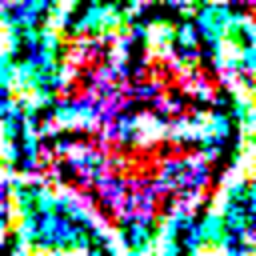
\includegraphics[width=\linewidth]{Images/AnPe/17_Einfahrtverbot} &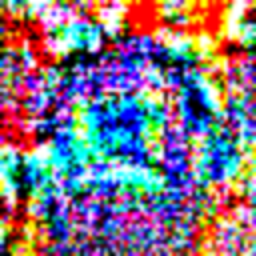
\includegraphics[width=\linewidth]{Images/AnPe/34_kreisverkehr_origTurnleft}  \\
	6.1a: Einfahrt verboten & 6.1b: Kreisverkehr \\
	99,99\% Konfidenz&95,35\% Konfidenz\\
	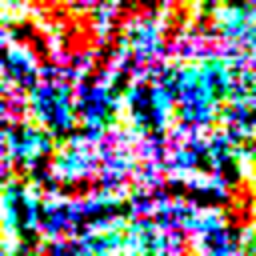
\includegraphics[width=\linewidth]{Images/AnPe/39_RechtsVorbeiOrigLinksvorbei} &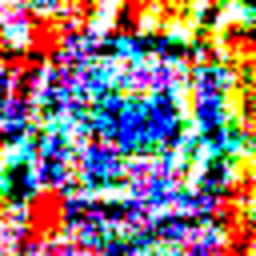
\includegraphics[width=\linewidth]{Images/AnPe/40_kreisverkehr}  \\
	6.1c: Rechts Vorbei&6.1d: Kreisverkehr\\
	99,50\% Konfidenz&98,68\% Konfidenz\\
\end{tabular}

\caption{Ergebnisse mit dem \textit{Gradient Ascent}-Verfahren (\textit{Targeted Backpropagation})}
\label{tab:gasc1}
\end{table}

